\documentclass[12pt,fleqn]{article}
\setlength{\parindent}{0pt}
\usepackage{graphicx}
\usepackage{cancel}
\usepackage{listings}
\usepackage[latin5]{inputenc}
\usepackage{color}
\setlength{\parskip}{8pt}
\setlength{\parsep}{0pt}
\setlength{\headsep}{0pt}
\setlength{\topskip}{0pt}
\setlength{\topmargin}{0pt}
\setlength{\topsep}{0pt}
\setlength{\partopsep}{0pt}
\setlength{\mathindent}{0cm}
\usepackage{latexsym}
\usepackage{showkeys}
\renewcommand*\showkeyslabelformat[1]{(#1)}

\begin{document}
Ders 20

Konumuz Laplace Transformu ile diferansiyel denklem cozmek. Fakat onu
yapmadan once, Laplace Transformunun mumkun oldugundan emin olmamiz
gerekiyor. Bazilariniz dusunebilir, ``ama hocam alttaki formul her zaman
hesaplanaz mi?''

\[ F(s) = \int_0^{\infty} f(t)e^{-st} \ dt \]

Cevap hayir cunku ustteki bir uygunsuz (improper) entegral, ust sinir
sonsuzluga gidiyor ve bildigimiz gibi uygunsuz entegraller her zaman bir
degere yaklasmiyorlar (converge). 

Laplace tranformunun mumkun olmasinin kontrolu, entegre edilen $f(t)$'nin
``cok hizli buyumemesi''yle alakali. Fonksiyonun buyuyebilir tabii,, ama
cok hizli buyurse o zaman $e^{-st}$ ile carpilmak onu asagi cekemez, ve
entegralin tamami bir degere yaklasamaz. O zaman $f(t)$'nin olmasi
gerektigi sarti ``ustel tipte (exponential type)'' olarak tarif
edebiliriz. Yani 

\[ |f(t)| \le C e^{kt}, \ \textit{ sabit } C > 0, \forall t \ge 0 
\textit{ herhangi bir } k > 0
\]

$f(t)$'nin kesin (absolute) degerini kullandik, fonksiyonun eksi yonde mi,
arti yonde mi oldugu onemli degil, onemli olan buyuyus (ya da kuculus)
hizi. Bu arada, ustteki tanimda bir suru dehset hizla buyuyen fonksiyon
mumkun, mesela $e^{100t}$'yi dusunelim; bu fonksiyonun nasil buyudugunu
goren var mi? Roket gibi yukari firlar, o kadar hizli bir buyumeden
bahsediyoruz. Yani ustteki sart genis bir yelpazedeki fonksiyonlari
kapsayabilir, cok kisitlayici sayilmaz. Bazi ornekler gorelim.

$sin(t)$ ustel tipte midir? Evet, cunku $|sin(t)| \le 1$ daha dogrusu
$|sin(t)| \le 1 \cdot e^{0t}$. 

Ya $t^n$? Bu fonksiyon da roket gibi yukari firlar ama acaba
karsilastirilacak ustel fonksiyonda $k$'yi yeterince buyuk yaparsak onun
ustesinden gelebilir miyiz? Sasirtici gelebilir ama buna gerek yok, $k=1$
bu isi hallediyor. 

\[ t^n \le M e^t, \ \textit{ M herhangi bir sabit }, \forall t > 0 \]

Yani bu ustel tip bir fonksiyon. Bunun tabii ki boyle olacagini tahmin
edebilirdik, gecen derste $t^n$'nin Laplace tranformunu hesapladik ne de
olsa (Laplace tranformu yapabilmek teoride her zaman ustel tip olmasi
anlamina gelmiyor aslinda, ama pratikte her zaman oyle), neyse, ama ustteki
karsilastirma nasil isledi? Su hesabi yapalim

\[ \frac{t^n}{e^t} \]

Iddia ediyorum ki ustteki ifade bir $M$ sabiti ile ``sinirlanmistir
(bounded by)'', yani hep $M$'in altindadir. Kontrol etmek icin yani

\[ \frac{t^n}{e^t} \le  M\]

sorusunu kontrol ederiz. Ya da onunla direk ilgili bir soru  $t \to \infty$ iken

\[ \frac{t^n}{e^t} \to ?\]

sorusunu. Ustteki bolum sifira yaklasir. Niye? Yine onceki dersten,
L'Hospital Kurali sebebiyle! Bolumun sifira gitmesi ne anlama gelir? 

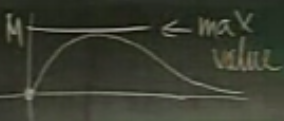
\includegraphics[height=2cm]{20_1.png}

Bolum sifirda baslamistir, ve sifira gider, ve surekli bir fonksiyondur. Bu
demektir ki arada bir yerde muhakkak bir maksimum degere (max value)
sahiptir, bu noktaya $M$ dersek, bolum $M$ tarafindan sinirlandirilmistir
diyebiliriz.

Simdi ustel tip ``olmayan'' iki tane fonksiyon gorelim. 

Mesela $1/t$ ustel tip degildir. 

\[ \int_0^{\infty} e^{-st}\frac{1}{t} dt  \]

Entegralin sinirlarina bakalim, $t$ 0 yakinda iken $e^{-st} \approx
1$. Geri kalan

\[ \int_0 \frac{dt}{t} \]

ki ust siniri belirtmedik, ne olursa olsun, bir noktaya yaklasmaz, ustteki
fonksiyon $ln(t)$ gibidir, $ln(0)=-\infty$ degeridir zaten. O zaman $1/t$
ustel tip degildir, ve $1/t$'nin Laplace tranformu yoktur. 

Bir bakima ustteki fonksiyon ``ise dogru baslamadigi'' icin ustel tip
olamamistir, tas bastan sonsuzluk devreye girmistir cunku. Daha ilginc bir
ornek asiri hizli buyuyen bir fonksiyon. Mesela

\[ e^{t^2} \]

Bu fonksiyon ustel tip olamayacak kadar hizli buyur. Cunku 

\[ e^{t^2} > e^{kt} \]

$k$ ne kadar buyuk olursa olsun ustteki ibare gecerlidir. 

Cunku sonsuza giderken $t^2 > kt$ olur, $t>k$'yi gectikten sonra bu
olacaktir, evet oraya gelinceye kadar bayagi beklemek gerekebilir, ama
sonsuza giderken bu kesinlikle olur.

E o zaman $e^{t^2}$ iceren diferansiyel denklemleri nasil cozecegiz?
Laplace ile degil ama baska bir sekilde. Nasil bir yol takip etmeliyiz?
Cozumu biz vermeyecegiz, cunku arastirmalarimizda oyle bir denklem hic
karsimiza cikmiyor. Tabiat sin, cos, $e$ iceren ustel fonksiyonlari
sever, fizikte $e^{t^2}$ turunden hicbir ifade gormedim, belki bu benim
cahilligimle alakali. 

Not: $e^{-t^2}$ baska bir hikaye. O y ekseninden asagi, iki yana yayilan bir
fonksiyon uretir. 

* * * 

Simdi Laplace Tranform ile diferansiyel denklem cozmeye gelelim. 

Laplace ile cozmek ve simdiye kadar kullandigimiz yontemlerle cozmek
arasinda cok temel bazi farkliliklar var. 

\[ y'' + Ay' + By = h(t) \]

Simdiye kadar gordugumuz teknikler bu problemi bu haliyle cozerler. Ama
Laplace tranformu bir baslangic sart problemine (initial value problem)
ihtiyac duyar. Yani cozumden once baslangic sartini kesinlikle tanimlamaniz
gerekir. 

Peki bu degerleri bilmiyorsam ne yaparim? O degerler icin degiskenler
atariz, 

\[ y(0) = y_0, \ y'(0) = y_0' \]

ve boyle devam ederiz, cozumun icinde tabii ki $y_0,y_0'$ degerleri
olacaktir. Yani bir anlamda baslangic degerleri yoksa bile ``varmis gibi''
yapiyoruz, kiyasla diger yontemlerde varmis gibi yapmaya bile gerek
yoktu. Kimisine gore bu buyuk bir eksik sayilabilir belki, kimisi icin de
hic onemli degildir. Biz ikinci bakis acisini bu derste takip edelim
isterseniz.

Bir turevin Laplace Tranformunu nasil yaparim? Bir turevin Laplace'i
{\em cebirsel} bir fonksiyondur, yani kendisi turev olmayan, dogaustu
(transcendental) olmayan bir $Y(s)$ fonksiyonu. 

$Y(s)$ elde edilince, onu cebirsel yontemlerle cozeriz. Her cebirsel
fonksiyon cozulebilir demiyoruz, ama Laplace'in bize sagladigi cebirsel
fonksiyonlar cozulebilir olacaktir. $Y$ fonksiyonlari polinomlar icerirler, 

\[ Y = \frac{p(s)}{q(s)} \]

$Y$'yi elde edince ne yapariz? Bu cozumun Laplace tranformudur, onu alip
$\mathcal{L}^{-1}$ ile geriye gideriz ve aradigimiz $y = y(t)$'yi buluruz. 

ODE'den cozume gitmek yerine ekstra Laplace basamagindan gecmek, sonra
geriye gitmek acaip gibi gelebilir, ama cogu zaman ODE'den direk cozume
gitmek zor oluyor, fakat $Y(s)$'ten bir cebirsel cozume ulasmak kolay
oluyor. Zaten tranformun kendisi de kolay. Tabii ters Laplace biraz zor,
kismi kesirler kullanilacak, tabloya bakilacak, vs. 






























\end{document}
